\documentclass[border=3pt]{standalone}
\usepackage{fontspec}
\usepackage{unicode-math}
\setmainfont{texgyretermes}[Extension=.otf, UprightFont=*-regular, BoldFont=*-bold,
  ItalicFont=*-italic, BoldItalicFont=*-bolditalic]
\setsansfont{texgyreheros}[Extension=.otf, UprightFont=*-regular, BoldFont=*-bold]
\setmathfont{texgyretermes-math.otf}
\newfontfamily\chessfont{Apple Symbols}
\usepackage{tikz}
\usepackage{pgfplots}
\pgfplotsset{compat=1.17}
\definecolor{light}{HTML}{EDEDED}
\definecolor{dark}{HTML}{7389B8}
\definecolor{edge}{HTML}{4A4A4A}
\definecolor{blue2}{HTML}{B9C6E0}
\begin{document}
\fontsize{8}{9.6}\selectfont
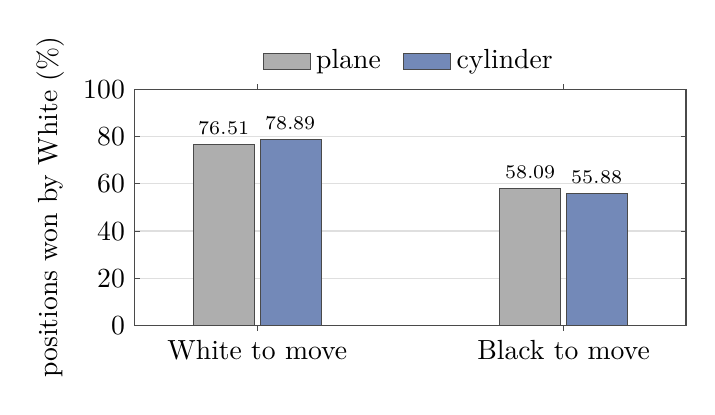
\begin{tikzpicture}\begin{axis}[ybar, bar width=22.0pt, scale only axis, width=7.0cm,
  height=3.0cm, ymin=0, ymax=100, ylabel={positions won by White (\%)}, symbolic x coords={White to move,Black to move}, xtick=data,
  ymajorgrids, grid style={gray!25}, enlarge x limits=0.40, area legend,
  legend style={at={(0.5,1.02)}, anchor=south, legend columns=-1, draw=none,
    /tikz/every even column/.append style={column sep=6pt}},
  axis line style={edge}, tick style={edge}, major tick length=2pt, nodes near coords, nodes near coords style={font=\fontsize{7}{7}\selectfont}]
\addplot[fill=edge!45, draw=edge, line width=0.3pt] coordinates {(White to move,76.51) (Black to move,58.09)};
\addlegendentry{plane}
\addplot[fill=dark, draw=edge, line width=0.3pt] coordinates {(White to move,78.89) (Black to move,55.88)};
\addlegendentry{cylinder}
\end{axis}\end{tikzpicture}
\end{document}
